% ====================================================================
%                                                                 
%
%       §06
%
%
% %%ts latex start%%[2019-03-07 Thu 14:45]%%ts latex end%%
% ====================================================================
% --------------------------------------------------------------------
% §1 Section <<Motivation>>
% --------------------------------------------------------------------



\begin{bem}[das Zeichen „$\Nz$“]
 In diesem Kapitel wird die Menge der natürlichen Zahlen, sofern die Null eingeschlossen ist, mit „$\Nz_0$“ bezeichnet, sofern die Null ausgeschlossen ist mit „$\Nz_{\geq 1}$“. In Situationen, in denen es keine Rolle spielt, ob die Null nun dabei ist oder nicht, schreiben wir einfach nur „$\Nz$“.
\end{bem}



\section{Zahlenfolgen}

\begin{de}[Folge] \label{folge}
Eine \textbf{Folge} ist eine Familie von Objekten $(a_n)_{n\in \Nz}$, deren Indexmenge die Menge $\Nz$ der natürlichen Zahlen ist. Ist $n\in \Zz$ eine beliebige ganze Zahl, so spricht man auch bei Familien, deren Indexmenge $\Zz_{\geq n}$ ist, von Folgen. In diesem Fall starten die Indizes nicht bei Eins oder Null, sondern bei $n$. Der Begriff der Folge ist also nicht klar umrissen, spricht man aber von „der beliebigen Folge $(a_n)$“ so ist damit gemeint, dass die Indexmenge gleich $\Nz$ (mit oder ohne Null) ist. \\
Sind $A$ eine Menge und $(a_n)_{n\in \Nz}$ eine Folge, deren Einträge allesamt in $A$ liegen, so spricht man von einer \emph{Folge von Elementen aus $A$} oder einer „$A$-wertigen Folge“. Nach \cref{familie} bezeichnet
\[ A^\Nz := \{ (a_n)_{n\in \Nz} \mid \forall n\in \Nz: a_n\in A \} \]
die Menge aller Folgen mit Einträgen aus $A$. Im Spezialfall $A=\Rz$ spricht man von \textbf{reellen Zahlenfolgen} oder auch \textbf{reellwertigen Folgen}. Analog spricht man von rationalen Zahlenfolgen, Folgen ganzer Zahlen oder Folgen komplexer Zahlen, falls es sich um Elemente von $\Qz^\Nz$, $\Zz^\Nz$ oder $\Cz^\Nz$ handelt. \\
Folgen lassen sich sowohl durch eine exakte Angabe definieren, etwa
\begin{align*}
  (n^2)_{n\in \Nz_0}
\end{align*}
als auch durch eine suggestive Aufzählung der ersten paar Folgenglieder, etwa
\[ 0,\quad 1,\quad 4,\quad 9,\quad 16,\quad 25,\quad\dots \]
Die „Definition durch Auflistung“ ist allerdings nicht mathematisch präzise und sollte nur dann benutzt werden, wenn wirklich unmissverständlich klar ist, welche Folge gemeint ist. Würdest du etwa erahnen, dass mit
\[ 0,\quad 2,\quad 12,\quad 36,\quad 80,\quad 150,\quad 252,\quad 392,\quad \dots\]
die Zahlenfolge $(n^2\cdot (n+1))_{n\in \Nz_0}$ gemeint sein soll?
\end{de}



\begin{bem}[Folge vs. Menge ihrer Einträge]
 Eine Folge $(a_n)_{n\in \Nz}$ ist nicht mit der Menge ihrer Einträge $\{a_n\mid n\in \Nz\}$ zu verwechseln.\footnote{vgl. \cref{mengeeinerfamilie}} Beispielsweise sind die beiden Zahlenfolgen
 \begin{align*}
  0,\quad 1,\quad 0,\quad 1,\quad 0,\quad \dots \\
  1,\quad 0,\quad 0,\quad 0,\quad 0,\quad \dots 
 \end{align*}
 voneinander verschieden, während die Mengen ihrer Einträge übereinstimmen und gleich der Menge $\{0,1\}$ sind.
\end{bem}



\begin{bsp}
 Beispiele für reelle Zahlenfolgen sind:
 \begin{enumerate}[a)]
  \item Die Folge der Primzahlen $2,3,5,7,11,\dots$. Also die Folge $(a_n)_{n\in \Nz_{\geq 1}}$ wobei für jedes $n\in \Nz_{\geq 1}$ mit $a_n$ die $n$-te Primzahl gemeint ist.
  \item Die Folge der natürlichen Zahlen $(n)_{n\in \Nz_0}$: $0,1,2,3,4,\dots$.
  \item Die Folge $0,1,-1,2,-2,3,-3,4,\dots$. Sie lässt sich definieren als diejenige Folge $(a_n)_{n\in \Nz_0}\in \Nz_0^{\Nz_0}$ mit den Einträgen
  \begin{align*}
  a_n := \begin{cases}
        -\frac{n}{2} & n\ \text{ist eine gerade Zahl} \\
        \frac{n+1}{2} & n\ \text{ist eine ungerade Zahl}
           \end{cases} && n \in \Nz_0
\end{align*}
  \item Die „alternierende Folge“ $((-1)^n)_{n\in \Nz_0}$. Also $1,-1,1,-1,1,-1,1,\dots$.
  \item Die Folge der Kehrwerte natürlicher Zahlen $(1/n)_{n\in \Nz_{\geq 1}}$. Das ist  $1,\frac{1}{2},\frac{1}{3},\frac{1}{4},\frac{1}{5},\dots$. Beachte, dass bei dieser Folge die Indizes erst bei Eins losgehen.
  \item Die Folge $\left(\frac{n}{n+1}\right)_{n\in \Nz_0}$. Also $0,\frac{1}{2},\frac{2}{3},\frac{3}{4},\frac{4}{5},\dots$.
  \item Die „konstante Folge“ $(3)_{n\in \Nz}$. Also: $3,3,3,3,3,\dots$.
  \item Für $q\in \Rz$ die Folge der $q$-Potenzen $(q^n)_{n\in \Nz_0}$ Im Fall $q=2$ erhielte man beispielsweise die Folge der Zweierpotenzen $1,2,4,8,16,\dots$.
 \end{enumerate}
In all diesen Beispielen gehorchen die Folgenglieder einer einfachen Regel. Dies muss aber nicht immer der Fall sein. Eine Folge darf auch völlig chaotisch sein und ihre Einträge brauchen keinem Muster zu gehorchen. Möglichst chaotische Folgen können mit einem Zufallsgenerator erzeugt werden. \\
Hier ist noch ein Beispiel für eine Folge, deren Einträge mal keine Zahlen sind:
\begin{itemize}
 \item Die Folge $(\{1,\dots , n\})_{n\in \Nz_0}$, deren Einträge die „Anfangsstücke“ von $\Nz_{\geq 1}$ sind. Also
 \[ \emptyset,\quad \{1\},\quad \{1,2\},\quad \{1,2,3\},\quad \{1,2,3,4\}\quad,\dots \]
 Dies ist keine Zahlenfolge, sondern eine Folge von Mengen. Sie besitzt die Eigenschaft, dass für jedes $n\in \Nz_0$ ihr $n$-ter Eintrag eine Menge ist, die genau $n$-viele Elemente enthält.
\end{itemize}
\end{bsp}



\begin{de}[Rechnen mit Folgen] \label{folgenrech}
Seien $(a_n)_{n\in \Nz}, (b_n)_{n\in \Nz}\in \Rz^\Nz$ zwei reelle Zahlenfolgen. Dann heißt die Folge
\[ (a_n)_{n\in \Nz}+(b_n)_{n\in \Nz} := (a_n + b_n)_{n\in \Nz} \]
die \textbf{Summe} von $(a_n)_{n\in \Nz}$ und $(b_n)_{n\in \Nz}$ und die Folge
\[ (a_n)_{n\in \Nz}\cdot (b_n)_{n\in \Nz}:= (a_n\cdot b_n)_{n\in \Nz} \]
heißt das \textbf{Produkt} der Folgen $(a_n)_{n\in \Nz}$ und $(b_n)_{n\in \Nz}$. \\
Ist ferner $\lambda\in \Rz$, so ist
\[ \lambda\cdot (a_n)_{n\in \Nz} := (\lambda\cdot a_n)_{n\in \Nz} \]
Da man Summe und Produkt zweier Zahlenfolgen dadurch erhält, dass man sie eintragsweise addiert bzw. multipliziert, spricht man auch von der \emph{komponentenweisen} Addition bzw. Multiplikation.
\end{de}


\begin{bsp}
Sind
\begin{align*}
 a_n & := (-1)^n \\
 b_n & := \frac{n}{n+1} && n \in \Nz_0
\end{align*}
so ist
\begin{align*}
 (a_n)_{n\in \Nz_0} + (b_n)_{n\in \Nz_0} & = \left((-1)^n+ \frac{n}{n+1}\right)_{n\in \Nz_0} &&= 1,\ \frac{-1}{2},\ \frac{5}{3},\ \frac{-1}{4},\ \frac{9}{5},\ \frac{-1}{6},\ \frac{13}{7},\dots \\
  (a_n)_{n\in \Nz_0} \cdot  (b_n)_{n\in \Nz_0} & = \left((-1)^n\cdot \frac{n}{n+1}\right)_{n\in \Nz_0} &&= 0,\ \frac{-1}{2},\ \frac{2}{3},\ \frac{-3}{4},\ \frac{4}{5},\ \frac{-5}{6},\ \frac{6}{7},\dots
\end{align*}
sowie
\begin{align*}
 3\cdot (b_n)_{n\in \Nz_0} & = \left( \frac{3n}{n+1}\right)_{n\in \Nz_0} && =0,\ \frac{3}{2},\ \frac{6}{3},\ \frac{9}{4},\ \frac{12}{5},\ \frac{15}{6},\dots \\
 0\cdot (a_n)_{n\in \Nz_0} & = \left(0\cdot (-1)^n\right)_{n\in \Nz_0} && = 0,0,0,0,0,\dots
\end{align*}

\end{bsp}



\begin{de}[Beschränktheit]
 Eine reelle Zahlenfolge $(a_n)_{n\in \Nz}\in \Rz^\Nz$ heißt \textbf{nach oben beschränkt} bzw. \textbf{nach unten beschränkt}, falls die Menge ihrer Einträge $\{a_n\mid n\in \Nz\}$ eine nach oben bzw. nach unten beschränkte Teilmenge von $\Rz$ im Sinne von \cref{schranken} ist. Konkret ist die Folge $(a_n)_{n\in \Nz}$ also genau dann
 \begin{itemize}
  \item \textbf{nach oben beschränkt}, falls es eine Zahl $M\in \Rz$ gibt, sodass $a_n\leq M$ für alle $n\in \Nz$ ist. In diesem Fall heißt ein solches $M$ eine \textbf{obere Schranke} für $(a_n)_{n\in \Nz}$.
  \item \textbf{nach unten beschränkt}, falls es eine Zahl $M\in \Rz$ gibt, sodass $a_n\geq M$ für alle $n\in \Nz$ ist. In diesem Fall heißt ein solches $M$ eine \textbf{untere Schranke} für $(a_n)_{n\in \Nz}$.
  \item \textbf{beschränkt}, falls sie sowohl nach oben als auch nach unten beschränkt ist.
  \item \textbf{unbeschränkt}, wenn sie nicht beschränkt ist.
 \end{itemize}
\end{de}


\begin{bsp} Es gilt:
\begin{itemize}
\item Die Folge $\left(\frac{n}{n+1}\right)_{n\in \Nz}$ ist nach unten durch $0$ und nach oben durch $1$ beschränkt.
\item Die Folge $2,3,5,7,11,\dots$ der Primzahlen ist nach oben unbeschränkt. Dies ist die Aussage des berühmten \emph{Satzes von Euklid}, siehe \cref{euklid}.
 \item Die alternierende Folge $((-1)^n)_{n\in \Nz}$ ist beschränkt, da sie nach oben durch $1$ und nach unten durch $-1$ beschränkt ist.
\end{itemize}
\end{bsp}



\begin{bem}
 Da die Beschränktheit einer Folge allein von der Menge ihrer Einträge abhängt, ist sie unempfindlich gegenüber einer Änderung der Reihenfolge der Folgeneinträge. Da beispielsweise die Folge
 \[ 0,\quad\frac{1}{2},\quad\frac{2}{3},\quad\frac{3}{4},\quad\frac{4}{5},\quad\frac{5}{6},\quad\frac{6}{7},\quad\dots \]
 nach unten durch $0$ und nach oben durch $1$ beschränkt ist, gilt dasselbe auch für die Folge
  \[ \frac{1}{2},\quad 0,\quad \frac{3}{4},\quad\frac{2}{3},\quad\frac{5}{6},\quad\frac{4}{5},\quad\frac{7}{8}\quad\dots \]
 die man durch eine Umordnung der Folgenglieder erhält.
\end{bem}


\begin{de}[Monotonie]
  Eine Folge reeller Zahlen $(a_n)_{n\in \Nz}\in \Rz^\Nz$ heißt
  \begin{itemize}
   \item \textbf{(monoton) wachsend}, falls für jedes $n\in \Nz$ gilt, dass $a_{n+1}\geq a_n$.
   \item \textbf{(monoton) fallend}, falls für jedes $n\in \Nz$ gilt, dass $a_{n+1}\leq a_n$.
   \item \textbf{monoton}, falls sie wachsend oder fallend ist.
  \end{itemize}
Gilt sogar $a_{n+1}>a_n$ für alle $n\in \Nz$, so sagt man auch, die Folge sei \emph{strikt wachsend}. Ähnlich definiert man auch „strikt fallend“.
\end{de}



\begin{bsp} Es gilt:
\begin{enumerate}[a)]
 \item Die alternierende Folge $((-1)^n)_{n\in \Nz}$ ist nicht monoton, da zum Beispiel $(-1)^3< (-1)^4$ aber auch $(-1)^4>(-1)^5$.
 \item Die Folge $\left(\frac{n}{n+1}\right)_{n\in \Nz}$ ist strikt wachsend.
 \begin{bew}
Für jedes $n\in \Nz$ ist
 \begin{align*}
  \frac{(n+1)}{(n+1)+1} - \frac{n}{n+1} & = \frac{(n+1)^2- n\cdot (n+2)}{(n+2)(n+1)} \\
  & = \frac{1}{(n+2)(n+1)} \\
  & >0
 \end{align*}
sodass $\frac{(n+1)}{(n+1)+1} > \frac{n}{n+1}$ ist. \qed
\end{bew}
 \item Für $q\in \Rz_{\geq 1}$ ist die Folge $(q^n)_{n\in \Nz}$ monoton wachsend.
 \begin{bew}
  Weil für jedes $n\in \Nz$ gilt:
  \begin{align*}
   q^{n+1} & = q \cdot q^n \\
   & \geq 1 \cdot q^n && (\text{wegen $q\geq 1$ und $q^n>0$})\\
   & = q^n \qed
  \end{align*}
 \end{bew}
 \item Eine reelle Folge ist genau dann sowohl monoton wachsend als auch monoton fallend, wenn sie konstant ist, d.h. wenn alle ihre Einträge identisch sind.
 \begin{bew}
  Sei $(a_n)_{n\in \Nz}\in \Rz^\Nz$ eine Folge, die gleichzeitig wachsend und fallend ist. Für jedes $n\in \Nz$ muss dann
  \[ a_{n+1}\geq a_n\qquad\text{und}\qquad a_{n+1}\leq a_n \]
  also insgesamt $a_{n+1}=a_n$ gelten. Aus der Tranitivität der Gleichheitsrelation\footnote{vgl. \cref{kettenfalten}} ergibt sich, das $a_n=a_0$ für jedes $n\in \Nz$ gilt. Also ist die Folge konstant. \qed
 \end{bew}
 \item Die Folge
 \[ 0,\quad -1,\quad -2,\quad -1,\quad 0,\quad 1,\quad 2,\quad 3,\quad 4, \quad 5,\dots \]
 ist nicht monoton. Sie könnte aber zu einer strikt wachsenden Folge gemacht werden, ließe man die ersten zwei Folgenglieder weg.
\end{enumerate}
\end{bsp}




\section{Abstand}

\begin{de}[Betrag und Abstand] \label{abstand}
Für eine reelle Zahl $a\in \Rz$ ist ihr \textbf{Betrag} definiert durch 
	\begin{align*}
		|a|=\begin{cases}
			a&a\geq 0\\
			-a&a<0
		\end{cases}
	\end{align*}
Beispielsweise ist
\[ \vert 3\vert = 3 \qquad\qquad \vert -7\vert =7 \qquad\qquad \vert 0\vert=0 \]
Sind $x,y\in \Rz$ zwei reelle Zahlen, so ist ihr \textbf{Abstand} definiert als
 \[ d(x,y) := \vert x -y\vert \]
 Beispielsweise ist
 \[ d(5,2)= 3 \qquad\qquad d(-2,5)=7 \qquad\qquad d(3,3)=0 \]
In der Literatur wird meistens der Buchstabe „$d$“ benutzt (für englisch ``distance'').
    \begin{figure}[H]
\begin{center}
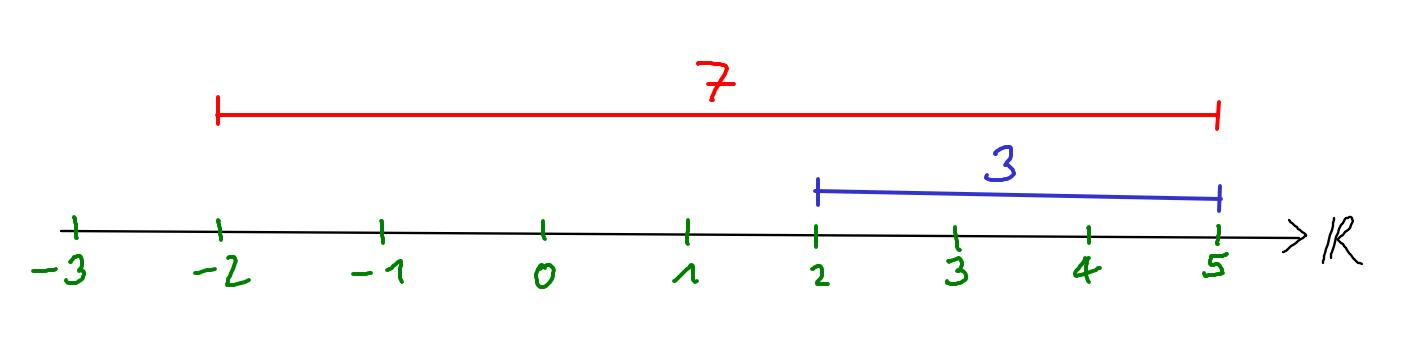
\includegraphics[width=12cm]{./_img/Abstand.jpeg}
\end{center}
\centering \caption{Abstände auf der reellen Gerade}
\end{figure}
\end{de}


\begin{bem}
Für jede reelle Zahl $x\in \Rz$ gilt:
 \[ \vert x\vert = \vert x-0\vert = d(x,0) \]
 d.h. der Betrag einer Zahl ist genau ihr Abstand zur Null.
\end{bem}



\begin{bem}[Allgemeine Abstände]
 In der Ebene $\Rz^2$, im Raum $\Rz^3$ und allgemein im Hyperraum $\Rz^n$ (für ein $n\in \Nz$) ist der Abstand zweier Punkte definiert als die Länge ihrer Verbindungsstrecke. Dies wird in den Analysis-Vorlesungen rigoros definiert werden, wir werden es hier aber ab und zu schon in einem informellen Sinn ausnutzen, um nette Beispiele und Illustrationen beisteuern zu können. Alle präzisen Aussagen und Beweise in diesem Text handeln aber lediglich von reellen Zahlen.
\end{bem}





\begin{de}[Intervalle in $\Rz$]
 Seien $a,b\in \Rz$ mit $a\leq b$. Dann heißen
 \begin{itemize}
  \item $(a,b) := \{ x\in \Rz \mid a<x<b \}$ das \textbf{offene Intervall} mit den Randpunkten $a$ und $b$. 
  \item $[a,b] := \{ x\in \Rz \mid a\leq x\leq b \}$ das \textbf{abgeschlossene Intervall} mit den Randpunkten $a$ und $b$.
  \item Die Mengen $[a,b) := \{ x\in \Rz \mid a\leq x<b \}$ und $(a,b] := \{ x\in \Rz \mid a<x\leq b \}$ heißen \textbf{halboffene Intervalle} mit Randpunkten $a,$ und $b$. 
 \end{itemize}
\end{de}



\begin{bem}
 Das offene Intervall $(a,b)$ besteht also aus genau denjenigen Elementen, die zwischen $a$ und $b$ liegen. Es ist nicht zu verwechseln mit dem Paar $(a,b)\in \Rz^2$. Da sowohl für das Paar $(a,b)\in \Rz^2$ als auch für das offene Intervall $(a,b)\subseteq \Rz$ dieselbe Notation verwendet wird, musst du beim Lesen mathematischer Texte aus dem Kontext erraten, von welchem Objekt gerade die Rede ist. \\[0.5em]
 Das abgeschlossene Intervall $[a,b]$ unterscheidet sich vom offenen Intervall $(a,b)$ lediglich dadurch, dass in $[a,b]$ auch noch die beiden „Randpunkte“ $a$ und $b$ enthalten sind, während sie bei $(a,b)$ fehlen.
\end{bem}



\begin{de}[offene Bälle]
 Für $x\in \Rz$ und $r\in \Rz_{\geq 0}$ ist der \textbf{offene Ball} um $x$ mit Radius $r$ definiert durch
 \[ \mathbb{B}_r(x) := \{ y\in \Rz \mid d(x,y)< r\} \]
$\mathbb{B}_r(x)$ besteht also genau aus denjenigen Elementen, deren Abstand zu $x$ kleiner als $r$ ist.
\end{de}


\begin{bsp}
 Für $x=4$ und $r= \frac{3}{2}$ ist
 \[ \mathbb{B}_{3/2}(4) = \left\{ y\in \Rz\mid \vert 4-y\vert <\frac{3}{2} \right\} = \left\{ y\in \Rz\mid 5/2<y<11/2 \right\} = \left(5/2,11/2\right) \]
    \begin{figure}[H]
\begin{center}
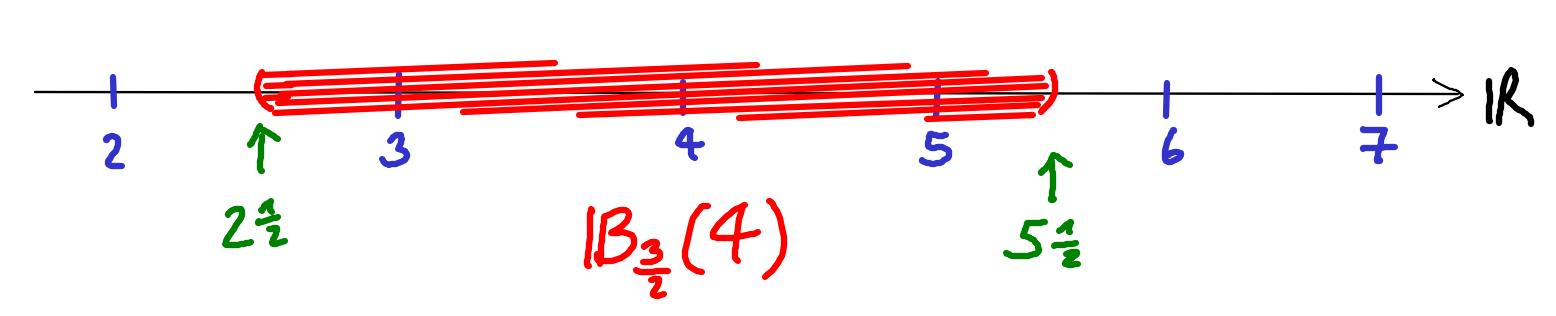
\includegraphics[width=10cm]{./_img/1Dball.jpeg}
\end{center}
\centering \caption{Der offene Ball $\mathbb{B}_{3/2}(4)$}
\end{figure}
 Dies sind genau die Punkte in $\Rz$, deren Abstand zur $4$ kleiner als $3/2$ ist. Allgemein gilt für reelle Zahlen $x\in \Rz$ und $r\in \Rz_{\geq 0}$:
 \[ \mathbb{B}_r(x) = (x-r,x+r) \]
\end{bsp}


\begin{bem}[Entartete Fälle]
Es gilt:
\begin{itemize}
 \item Sind $a,b\in \Rz$ mit $a=b$, so ist $(a,b)=(a,a)=\emptyset$, da es kein Element gibt, das sowohl strikt kleiner als auch strikt größer als $a$ wäre. Ebenso wären $[a,a)=(a,a]=\emptyset$, wohingegen $[a,a]=\{a\}$.
 \item Für jedes $x\in \Rz$ ist $\mathbb{B}_0(x)=\emptyset$, da es kein Element gibt, dessen Abstand zu $x$ noch kleiner als Null wäre.
\end{itemize}
\end{bem}



\begin{bem}[zum Wort „Ball“]
 Zugegeben ergibt die Bezeichnung „offener Ball“ auf der (eindimensionalen) Zahlengerade nicht so viel Sinn, da es sich dabei um Intervalle handelt. Sobald man aber in der Ebene $\Rz^2$ oder im Raum $\Rz^3$ unterwegs ist, sehen die „Bälle“ auch wirklich aus wie Bälle: \\[0.5em]
 In der Ebene $\Rz^2$ ist zum Beispiel der offene Ball $\mathbb{B}_{1}\begin{pmatrix} 2 \\ 1\end{pmatrix}$ gegeben durch: \\
    \begin{figure}[H]
\begin{center}
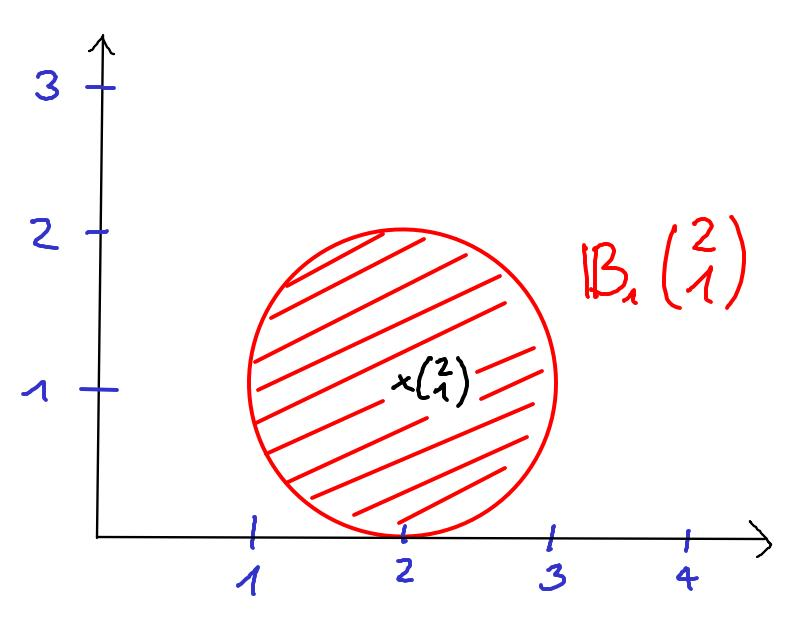
\includegraphics[width=10cm]{./_img/2Dball.jpeg}
\end{center}
\centering \caption{Menge aller Punkte in der Ebene $\Rz^2$, deren Abstand zum Punkt mit den Koordinaten $(2,1)$ kleiner als $1$ ist.}
\end{figure}
Im Raum $\Rz^3$ ist beispielsweise der offene Ball $\mathbb{B}_{2}\begin{pmatrix} 1\\ 1 \\ 1\end{pmatrix}$ gegeben durch: \\
    \begin{figure}[H]
\begin{center}
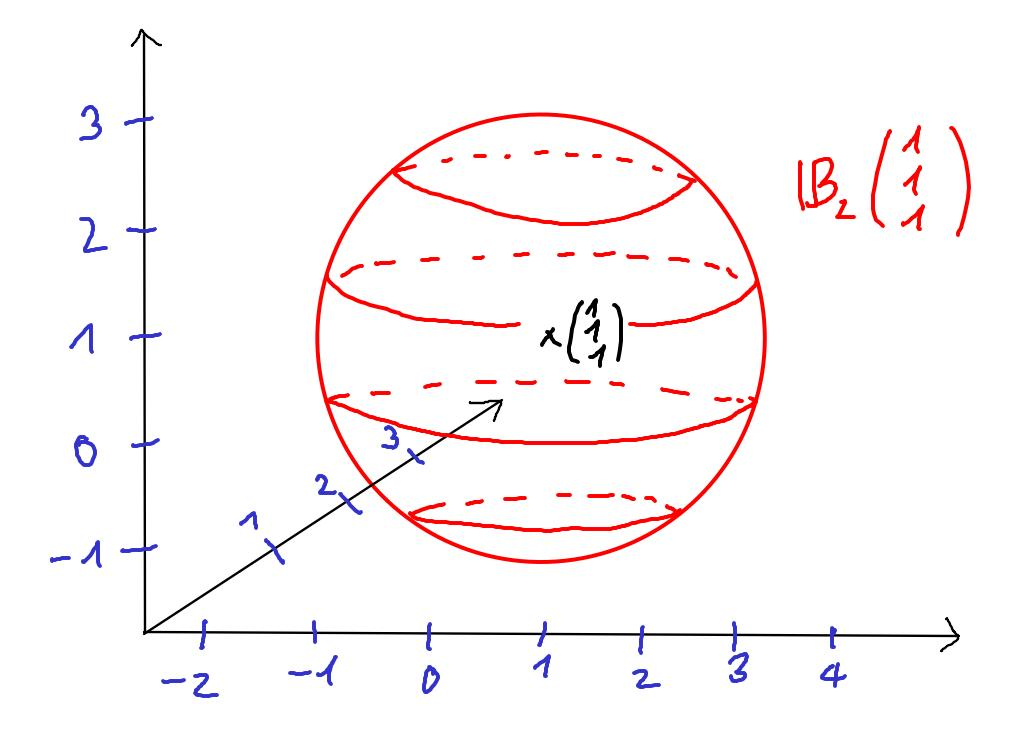
\includegraphics[width=10cm]{./_img/3Dball.jpeg}
\end{center}
\centering \caption{Menge aller Punkte im Raum $\Rz^3$, deren Abstand zum Punkt mit den Koordinaten $(1,1,1)$ kleiner als $2$ ist.}
\end{figure}
Beachte aber, dass diese offenen Bälle keinen „Rand“ haben. Denn $\mathbb{B}_r(x)$ besteht ja nur aus den Elementen, deren Abstand zu $x$ strikt kleiner als $r$ ist. Diejenigen Elemente, deren Abstand zu $x$ genau gleich $r$ ist (im Zweidimensionalen also genau die Punkte auf dem Kreisrand, im Dreidimensionalen die Punkte auf der Kugeloberfläche), sind nicht in $\mathbb{B}_r(x)$ enthalten.
\end{bem}




\begin{comment}
\begin{sat}
	Für $x,y\in\Rz$ gilt
	\begin{resListeN}
		\item $x=0\lra |x|=0$
		\item $x\leq |x|$
		\item $|xy|=|x||y|$
		\item $|x+y|\leq |x|+|y|$
	\end{resListeN}
\end{sat}
\begin{bew}
	\begin{bewListeN}
		\item folgt direkt aus der Definition
		\item für $x\geq 0$ gilt $x=|x|$. Im anderen Fall folgt $x<0<-x=|x|$
		\item Für $x=0\vee y=0$ ist die Aussage trivial. Seien also $x,y\neq 0$.
			\begin{itemize}
				\item[$x,y>0$:] damit ist auch $xy>0$. Also: $|xy|=xy=|x||y|$
				\item[$x,y<0$:] auch hier ist $xy>0$. Das heißt $|xy|=xy=(-x)(-y)=|x||y|$
				\item[$x<0,y>0$:] hier ist $xy<0$ und damit $|xy|=-xy=(-x)y=|x||y|$.
				\item[$x>0,y<0$:] analog
			\end{itemize}
		\item Da beide Seiten positiv sind, ist das Quadrieren eine Äquivalenzumformung. Dann folgt mit ii)
			\begin{align*}
				|x+y|\leq |x|+|y|\lra x^2+2xy+y^2\leq x^2+2|xy|+y^2\lra 2xy\leq 2|xy|
			\end{align*}
	\end{bewListeN}
\bewEnd
\end{bew}
\end{comment}


% --------------------------------------------------------------------
% §3 Section <<Konvergenz>>
% --------------------------------------------------------------------
\section{Konvergenz}

\begin{bem}[Motivation]
 Betrachten wir einmal eine Folge von Punkten in der Ebene, sie sich spiralenförmig dem Ursprung annähert:
     \begin{figure}[H]
\begin{center}
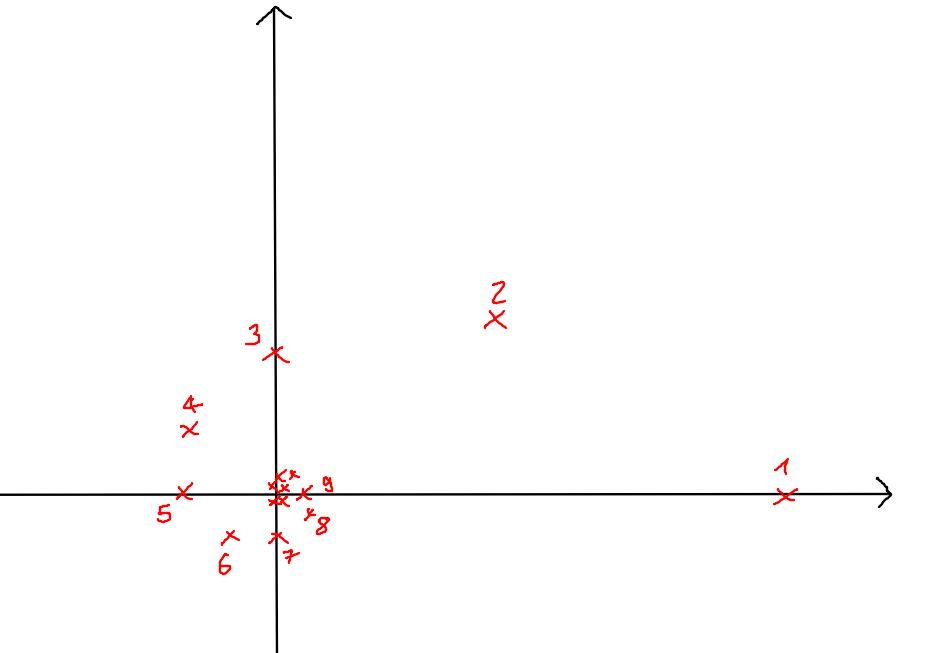
\includegraphics[width=10cm]{./_img/Spirale.jpeg}
\end{center}
\centering \caption{Eine konvergente Folge von Punkten in der Ebene}
\end{figure}
Konkret könnte man
\begin{align*}
 a_n & := \frac{1}{n}\cdot \begin{pmatrix}
           \cos(n\cdot \pi/4) \\
           \sin(n\cdot \pi/4)
          \end{pmatrix} && n\in \Nz
\end{align*}
definieren, aber das soll gerade keine Rolle spielen. \\
Man sieht, dass die Folgenglieder dem Koordinatenursprung immer näher kommen, sich ihm geradezu „anschmiegen“.
\end{bem}



Dass eine Folge gegen einen Grenzwert konvergiert, heißt grob gesagt, dass sie diesem Grenzwert „irgendwann beliebig nahe kommt“. Die übliche mathematische Formalisierung dieser Vorstellung geht folgendermaßen:
\begin{de}[Konvergenz]
	Seien $(a_n)_{n\in \Nz}\in \Rz^\Nz$ eine Folge reeller Zahlen und $a\in \Rz$. Man sagt, die Folge $(a_n)_{n\in \Nz}$ \textbf{konvergiert} gegen $a$, falls es für jedes $\varepsilon \in \Rz_{>0}$ ein $N\in \Nz$ gibt, sodass ab dem $N$-ten Folgenglied alle Folgenglieder in $\mathbb{B}_\epsilon(a)$ liegen. Als Quantorenformel:
	\begin{align*}
	\forall\epsilon\in \Rz_{>0}\ \exists N\in\Nz\ \forall n\in \Nz_{\geq N}:\ a_n\in \mathbb{B}_\epsilon(a)
	\end{align*}
	In diesem Fall heißt $a$ ein \textbf{Grenzwert} der Folge $(a_n)_{n\in \Nz}$. Man schreibt
	\[ \limm{n\longra\infty}a_n=a \qquad\text{oder}\qquad a_n\xrightarrow[n\to \infty]{} a \]
	Eine Folge, die keinen Grenzwert besitzt, heißt \textbf{divergent}.
\end{de}



\begin{bem}[„Sei $\epsilon>0$“]
 Diese Grenzwertdefinition ist vergleichsweise jung: sie stammt aus dem 19. Jahrhundert und wurde durch Cauchy\footnote{\href{https://de.wikipedia.org/wiki/Augustin-Louis_Cauchy}{Augustin-Louis Cauchy (1789 - 1857)}} und Weierstraß\footnote{\href{https://de.wikipedia.org/wiki/Karl_Weierstra\%C3\%9F}{Karl Weierstraß (1815 - 1897)}} populär. Bis dahin herrschte in der Mathematik ein eher „intuitiver“ Umgang mit Grenzwerten vor. \\[0.5em]
 Seit dem Aufkommen der modernen Analysis hat es sich eingebürgert, in Definitionen und Beweisen jene Abstände, die „beliebig klein“ werden sollen, mit einem „$\epsilon$“ zu notieren. Aus diesem Grund spricht man bei Definitionen und Beweisen der Analysis, die viel Gebrauch von $\epsilon$'s machen, von „Epsilontik“.
\end{bem}





\begin{bsp}
 Die durch
 \begin{align*}
  a_n &:= \frac{n}{n+1} && n\in \Nz
 \end{align*}
 definierte reelle Folge $(a_n)_{n\in \Nz}\in \Rz^\Nz$ konvergiert gegen $1$.
\end{bsp}
     \begin{figure}[H]
\begin{center}
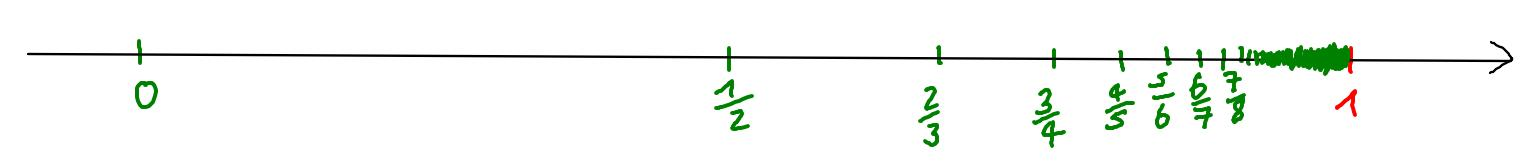
\includegraphics[width=14cm]{./_img/Konvergenzbsp.jpeg}
\end{center}
%\centering \caption{Eine konvergente Folge von Punkten in der Ebene}
\end{figure}
\begin{bem}
Bevor wir versuchen, für diese Aussage einen Bilderbuchbeweis hinzuschreiben, wollen wir „auf dem Skizzenblatt“ erstmal ein paar Überlegungen anstellen: \\
 Wir müssen für ein beliebiges $\varepsilon \in \Rz_{>0}$ ein $N\in \Nz$ finden, sodass für alle $m\in \Nz_{\geq N}$ gilt:
 \begin{align*}
   \epsilon &  > d(1,\frac{m}{m+1})
   \end{align*}
   Mit ein paar Umformungen ergibt sich:
   \begin{align*}
  d(1,\frac{m}{m+1}) & = \left| 1-\frac{m}{m+1}\right| \\
   & = \left| \frac{m+1}{m+1} - \frac{m}{m+1} \right| \\
   & = \left| \frac{1}{m+1}\right| \\
   & = \frac{1}{m+1} & (\text{da $m\in \Nz$})
 \end{align*}
Die Ungleichung $\epsilon >d(1,m/(m+1))$ lässt sich daher umformen zu
\[ m > \frac{1}{\epsilon} -1  \]
Wählen wir also für $N$ die nächstgrößere natürliche Zahl oberhalb von $1/\epsilon$, indem wir $1/\epsilon$ aufrunden (man könnte für $N$ auch jede weitere Zahl, die größer als $(1/\varepsilon -1)$ ist, verwenden). Dann sind sowohl $N$ als auch alle $m\in \Nz_{>N}$ größer als $1/\epsilon- 1$, sodass die Ungleichung aufgeht. \\[0.5em]
Damit haben wir die Aufgabe auf dem Schmierblatt gelöst. Im finalen Beweis lassen wir die Überlegungen, die uns zur Wahl von $N$ geführt haben, weg. Dies tritt häufig in Analysis-Beweisen auf: die Beweise unterdrücken den Gedankenprozess, der zu ihrem Auffinden geführt hat und verlaufen genau in die entgegengesetzte Richtung:
\end{bem}
\begin{bew}
Es sei $\varepsilon \in \Rz_{>0}$ beliebig. Sei $N\in \Nz$ die kleinste natürliche Zahl, die größer als $1/\epsilon$ ist. Für alle $m\in \Nz_{\geq N}$ gilt dann:
\begin{align*}
 d(1,a_m) & = \left| 1-\frac{m}{m+1}\right| \\
 & = \left| \frac{1}{m+1} \right| \\
 & = \frac{1}{m+1} \\
 & < \frac{1}{m} \\
 & \leq \frac{1}{N} & (\text{da $m\geq N$})\\
 & < \frac{1}{1/\epsilon} & (\text{da $N> 1/\epsilon$}) \\
 & = \epsilon
\end{align*}
Somit liegen ab dem $N$-ten Folgenglied alle Folgenglieder in $\mathbb{B}_\epsilon(1)$. Da $\epsilon \in \Rz_{>0}$ beliebig gewählt war, ist damit bewiesen, dass die $a_n$'s gegen $1$ konvergieren. \qed
\end{bew}



\begin{bem}
 Beachte, dass die Tatsache, ob eine Folge konvergiert oder divergiert, eine reine Eigenschaft des „Langzeitverhaltens“ dieser Folge ist. Die ersten paar Millionen Folgenglieder haben für sich allein keinen Einfluss auf das Konvergenzverhalten, weil die Folge ja ab dem dreimillionsten Eintrag plötzlich eine ganz andere Richtung einschlagen könnte. (Die Folgen, mit denen man es in der Praxis zu tun hat, unterliegen aber meist einem einfachen Muster, das spätestens nach ein paar Dutzend Folgengliedern ersichtlich sein sollte)
\end{bem}




\begin{bsp}
 Die Folge der Quadratzahlen $(n^2)_{n\in \Nz}$ besitzt keinen Grenzwert.
\end{bsp}
\begin{bew}
 Für einen Widerspruchsbeweis sei angenommen, es gebe einen Grenzwert $a\in \Rz$. Dann gäbe es ein $N\in \Nz$, sodass für alle $n\in \Nz_{\geq N}$ gälte, dass $n^2 \in \mathbb{B}_1(a)$. Wähle ein $k\in \Nz$, für das sowohl $k>N$ als auch $k^2>a+1$ gilt. Dann wäre $k^2\in \mathbb{B}_1(a)$ und wegen $\mathbb{B}_1(a)=(a-1,a+1)$ folgte der Widerspruch $a+1 < k^2 < a+1$. \qed
\end{bew}




\begin{bsp}[Konstante Folgen konvergieren]
 Sei $x \in \Rz$ beliebig. Dann konvergiert die konstante Folge $(x)_{n\in \Nz}$ gegen $x$.
 \[ x,x,x,x,\dots \qquad \xrightarrow[n\to \infty]{} x \]
\end{bsp}
\begin{bew}
Sei $\varepsilon \in \Rz_{>0}$ beliebig. Für jedes $n\in \Nz$ ist $\vert a_n-x\vert =x-x=0 < \varepsilon$. \qed
\end{bew}





\section{Einige Konvergenzgesetze}


\begin{sat}[Eigenschaften der Abstandsfunktion]
 Für alle reellen Zahlen $x,y,z \in \Rz$ gilt:
 \begin{align*}
  d(x,y)=0 \quad &\leftrightarrow\quad x=y && (\text{Definitheit}) \\
  d(x,y) & = d(y,x) && (\text{Symmetrie}) \\
  d(x,z) & \leq d(x,y)+d(y,z) && (\text{Dreiecksungleichung})
 \end{align*}
\end{sat}
\begin{bew}
 Wir werden diese Eigenschaften hier ohne Beweis verwenden. Einen Beweis kannst du z.B. in Satz I.11.4 im Analysis-Lehrbuch \citet{AE06} (das du über den Link im Literaturverzeichnis kostenlos aus dem Uni-Netz herunterladen kannst) nachschlagen. Du kannst aber auch abwarten, bis diese Eigenschaften in der Ana1-Vorlesung thematisiert werden.
\end{bew}



\begin{bem}[Metrische Räume]
 Die obigen drei Aussagen können auch an und für sich untersucht werden: Ist $X$ eine beliebige Menge und $d:X\times X\to \Rz_{\geq 0}$ eine Abbildung, die diese drei Aussagen erfüllt, so nennt man $d$ eine „Metrik“ und das Paar $(X,d)$ einen „\href{https://de.wikipedia.org/wiki/Metrischer_Raum}{metrischen Raum}“. Ein erheblicher Teil der Analysis reeller Zahlen verallgemeinert sich auf beliebige metrische Räume, was meist in der Zweitsemestervorlesung „Analysis 2“ thematisiert wird.
\end{bem}




\begin{bem}[zur Dreiecksungleichung]
 Der Name „Dreiecksungleichung“ ergibt, sofern man nur Abstände reeller Zahlen untersucht, nicht so viel Sinn. Vielmehr kommt er aus der ebenen bzw. räumlichen Geometrie. Sind $x,y,z\in \Rz^2$ drei Punkte in der Ebene, die ein Dreieck bilden, so besagt die Dreiecksungleichung, dass „der direkte Weg von $x$ nach $z$ nicht länger als der Umweg über $y$ sein kann“:
     \begin{figure}[H]
\begin{center}
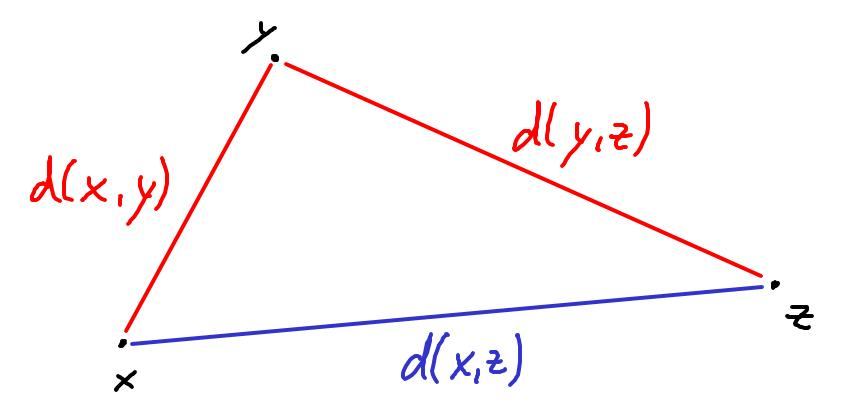
\includegraphics[width=10cm]{./_img/Dreiecksungleichung.jpeg}
\label{zahlenkugel}
%\centering \caption{Die Summe zweier Dreiecksseitenlängen ist stets kleiner als die Länge der dritten Seite.}
\end{center}
\end{figure}
\end{bem}





\begin{sat}[Eindeutigkeit des Grenzwerts]
 Sofern eine Folge reeller Zahlen konvergiert, ist ihr Grenzwert eindeutig bestimmt.
\end{sat}
\begin{bew}
Seien $(a_n)_ {n\in \Nz}\in \Rz^\Nz$ eine reelle Zahlenfolge, $a,b\in \Rz$ und es gelte sowohl $a_n\xrightarrow[n\to \infty]{} a$ als auch $a_n\xrightarrow[n\to \infty]{} b$. Ferner sei $\varepsilon \in \Rz_{>0}$. \\
Weil die $a_n$'s gegen $a$ konvergieren, gibt es ein $N\in \Nz$, sodass für alle $m\in \Nz_{\geq N}$ gilt, dass $a_m\in \mathbb{B}_{\varepsilon/2}(a)$. Und weil die $a_n$'s auch gegen $b$ konvergieren, gibt es ebenso ein $M\in \Nz$, sodass für alle $m\in \Nz_{\geq M}$ gilt, dass $a_m\in \mathbb{B}_{\varepsilon/2}(b)$. \\
Sei nun $k\in \Nz$ eine Zahl, die sowohl größer als $N$ als auch größer als $M$ ist. Dann gilt
\[ a_k \in \mathbb{B}_{\varepsilon/2}(a) \qquad\text{und}\qquad  a_k \in \mathbb{B}_{\varepsilon/2}(b) \]
Mit der Dreiecksungleichung folgt
\[ d(a,b) \leq d(a,a_k) + d(a_k,b) < \frac{\epsilon}{2}+\frac{\epsilon}{2} = \epsilon \]
Da die Zahl $\varepsilon\in \Rz_{>0}$ beliebig gewählt war, ergibt sich, dass der Abstand $d(a,b)$ kleiner als jede beliebige positive reelle Zahl sein muss. Damit bleibt nur noch $d(a,b)=0$ übrig, woraus aufgrund der Definitheit der Abstandsfunktion folgt, dass $a=b$. \qed
\end{bew}



\begin{bem}[\textbf{Der} Grenzwert einer Folge]
 Dieser Satz berechtigt uns, bei einer konvergenten Folge $(a_n)_{n\in \Nz}\in \Rz^\Nz$ anstelle von „einem Grenzwert“ von \emph{dem} Grenzwert dieser Folge zu sprechen. Ist $a\in \Rz$ der Grenzwert der $a_n$'s, so suggeriert die Notation
 \[ \lim_{n\to \infty} a_n = a \]
 ja auch schon, dass „$\lim_{n\to \infty}a_n$“ ein wohlbestimmtes Objekt ist, das eben gleich $a$ oder ungleich $a$ sein kann.
\end{bem}



%------------------
%3.10 Satz
\begin{sat}[Rechenregeln für Folgengrenzwerte]
	Seien $(a_n)_{n\in \Nz},(b_n)_{n\in \Nz}\in \Rz^\Nz$ zwei konvergente Folgen mit $a=\limm{n\longra\infty}a_n$ und $b=\limm{n\longra\infty}b_n$. Dann gilt:
	\begin{enumerate}[a)]
		\item $\limm{n\longra\infty}(a_n+b_n)=a+b$
		\item $\limm{n\longra\infty}(\lambda \cdot a_n)=\lambda \cdot a$ für $\lambda\in\Rz$
		\item $\limm{n\longra\infty}(a_n\cdot b_n)=a\cdot b$.
	\end{enumerate}
\end{sat}

%------------------
% 3.11 Beweis
\begin{bew}
Wir werden hier nur die Gleichung für die Addition beweisen. Die Punkte b) und c) werden in der Ana1-Vorlesung bewiesen werden\footnote{und lassen sich etwa in Satz II.2.2 und Satz II.2.4 im hervorragenden Lehrbuch \citet{AE06} nachschlagen.}. \\[0.5em] 
Sei $\epsilon \in \Rz_{>0}$ eine beliebige positive reelle Zahl. Weil die $a_n$'s gegen $a$ konvergieren, existiert ein $N\in\Nz$ sodass $a_n\in\mathbb{B}_{\epsilon/2}(a)$ für alle $n\in \Nz_{\geq N}$ gilt. Und weil die $b_n$'s gegen $b$ konvergieren, existiert ein $M\in \Nz$, sodass $a_n\in\mathbb{B}_{\epsilon/2}(b)$ für alle $n\in \Nz_{\geq M}$ gilt. Setze $K:=\max\{N,M\}$ auf die größere der beiden Zahlen $M,N$. Für alle $n\in \Nz_{\geq K}$ ist dann $a_n \in \mathbb{B}_{\epsilon/2}(a)\cap\mathbb{B}_{\epsilon/2}(b)$, sodass
    \begin{align*}
    \betrag{(a_n+b_n)-(a+b)}& = \vert (a_n-a) + (b_n-b)\vert \\
    & \leq \betrag{a_n-a}+\betrag{b_n-b } &&(\text{ohne Beweis})\\
    & <\frac{\epsilon}{2}+\frac{\epsilon}{2} &&(\text{da $a_n\in  \mathbb{B}_{\epsilon/2}(a)\cap\mathbb{B}_{\epsilon/2}(b)$})\\
    & =\epsilon
    \end{align*}
Da $\varepsilon\in \Rz_{>0}$ beliebig gewählt war, folgt, dass die Folge $(a_n+b_n)_{n\in \Nz}$ gegen $a+b$ konvergiert. \qed
\end{bew}



\begin{bem}[Komplizierte Objekte in einfache Bausteine zerlegen]
 Sätze wie dieser sind von herausragender Bedeutung für die Analysis. Sofern man einen kleinen Vorrat an Folgen, für die man ihre Konvergenz bewiesen hat, aufgebaut hat, erlauben sie es, Grenzwerte für die kompliziertesten Folgen auszurechnen, ohne dass man für einen Beweis nochmal die $\epsilon$'s auskramen müsste. \\
Beispielsweise würde kein routinierter Mathematiker einen $\epsilon$-Beweis dafür führen, dass die Folge
 \[ \left( 1 + \frac{3n}{n+1} \right)_{n\in \Nz} \]
 gegen $4$ konvergiert. Sondern er würde schlicht bemerken, dass sich diese Folge als Linearkombination
 \[ (1)_{n\in \Nz} + 3\cdot \left(\frac{n}{n+1}\right)_{n\in \Nz} \]
 zusammensetzt und dann auf die Rechenregeln für $\lim_{n\to\infty}(-)$ verweisen. Denn es ist
 \[ 4 = 1+3\cdot 1 = \left( \lim_{n\to \infty} 1 \right)+3\cdot \left( \lim_{n\to \infty} \frac{n}{n+1} \right) = \lim_{n\to \infty} \left( 1+ \frac{3n}{n+1} \right) \]
 Diese Denkweise kennst du auch aus der Schule: Um beispielsweise die Ableitung der Funktion
 \begin{align*}
  f(x) &= (x^2+3x)\cdot e^x && x\in \Rz
 \end{align*}
 zu berechnen, würdest du ausnutzen, dass sich diese Funktion aus den Bestandteilen
 \begin{align*}
  g(x)& = x^2 \\
  h(x) & = 3x \\
  q(x) &= e^x && x\in \Rz
 \end{align*}
 zusammensetzt via
 \begin{align*}
  f(x) & = (g(x)+h(x))\cdot q(x) && x\in \Rz
 \end{align*}
Mittels Summen- und Produktregel würdest du schlussfolgern
\begin{align*}
 f'(x) & = (g'(x)+h'(x))\cdot q(x)  + (g(x)+h(x))\cdot q'(x) \\
 & = (2x+3)\cdot e^x + (x^2+3x)\cdot e^x \\
 & = (x^2+5x+3)\cdot e^x && x\in \Rz
\end{align*}
Die „analytische“ Methode, komplexe Funktionen in einfache Bestandteile zu zerlegen, ist auch an der Uni überlebensnotwendig. Kein erfahrener Mathematiker würde, um die Ableitung von $(x^2+3x)\cdot e^x$ zu berechnen, unmittelbar mit der Definition der Ableitung arbeiten und versuchen, den Differenzialquotienten
\begin{align*}
 f'(x)&:=\limm{h\longra 0} \frac{((x+h)^2+3(x+h))\cdot e^{x+h} - (x^2+3x)\cdot e^{x}}{h} && x\in \Rz
\end{align*}
direkt auszurechnen. \\[0.5em]
Ein Ziel der Analysis-Vorlesung ist es, dich mit Werkzeugen auszustatten, die das Berechnen von Grenzwerten bequemer machen und Epsilontik vermeiden. Versuche in Analysis-Beweisen, die Objekte immer soweit es geht in einfachste Bausteine zu zerlegen und einen $\epsilon$-Beweis erst wenn gar nichts anderes mehr geht als Ultima Ratio anzusetzen.
\end{bem}






% --------------------------------------------------------------------
% §5 Section <<Aufgabenvorschlaege>>
% --------------------------------------------------------------------
\newpage
\section{Aufgabenvorschläge}

%Das hier sind die Übungsaufgaben zum Folgen-Vortrag im Vorkurs WS 2014.



% --------------------------------------------------------------------
% §5.1 Subsection <<Aufgabe 1>>
% --------------------------------------------------------------------






\begin{aufg}[Konkrete Folgen]
Untersucht jede der folgenden Folgen darauf, ob sie (nach oben oder unten) beschränkt und/oder monoton ist.
\begin{enumerate}[a)]
  \item Die Folge der Kehrwerte natürlicher Zahlen $(1/n)_{n\in \Nz_{\geq 1}}$. Das ist  $1,\frac{1}{2},\frac{1}{3},\frac{1}{4},\frac{1}{5},\dots$.
  \item Die Folge $(n^2)_{n\in \Nz}$ der Quadratzahlen: $0,1,4,9,16,\dots$.
  \item Die Folge $0,1,-1,2,-2,3,-3,4,\dots$.
  \item[d)*] Die Folge $(\sin(n))_{n\in \Nz}$.
\end{enumerate}
\end{aufg}





\begin{aufg}[Teilmengen skizzieren]
Visualisiert die folgenden Teilmengen von $\Rz$ jeweils durch eine Zeichnung:
\begin{align*}
 &\text{a)} && \bigcup_{k\in \Zz} [3k+1,3k+2] \\
&\text{b)} && \bigcup_{n\in \Nz} \left[ -n, \frac{n}{n+1} \right] \\
 &\text{c)} && \bigcap_{n\in \Nz_{\geq 1}} \mathbb{B}_{1/n}(7) \\
 &\text{d)*} && \bigcup_{n\in \Nz_{\geq 1}} \left( \bigcup_{k\in \Zz} \left[\frac{3k+1}{3^n},\frac{3k+2}{3^n} \right] \right)
\end{align*}
\end{aufg}





\begin{aufg}[Intuition für $\Rz$]
Beurteile intuitiv, ob die folgenden Aussagen wahr oder falsch sind. Du brauchst in dieser Aufgabe keine wasserdichten Beweise formulieren und dir auch nicht hundertprozentig sicher sein; es geht hier um die Schärfung deiner Intuition für reelle Zahlen.
\begin{enumerate}[a)]
 \item Sind $x,y,z\in \Rz$ mit $d(x,y)<2$ und $d(y,z)<3$, so ist $d(x,z)<5$.
 \item Sind $x,y,z\in \Rz$ mit $d(x,y)>2$ und $d(y,z)>3$, so ist $d(x,z)>5$.
  \item Jede monoton wachsende Folge reeller Zahlen konvergiert.
 \item Jede beschränkte, monoton wachsende Folge reeller Zahlen konvergiert.
  \item Jede konvergente Folge reeller Zahlen ist beschränkt.
 \item Jede beschränkte Folge reeller Zahlen konvergiert.
 \item Ist $(a_n)_{n\in \Nz}\in \Rz^\Nz$ eine konvergente Zahlenfolge und ist $a_n\leq 4$ für alle $n\in \Nz$, so ist auch $\lim_{n\to\infty} a_n\leq 4$.
 \item Ist $(a_n)_{n\in \Nz}\in \Rz^\Nz$ eine konvergente Zahlenfolge und ist $a_n <4$ für alle $n\in \Nz$, so ist auch $\lim_{n\to\infty} a_n<4$.
\end{enumerate}
\end{aufg}





\begin{aufg}[Konvergenzbeweis]
Zeigt mithilfe eines $\epsilon$-Beweises, dass die Folge $(2^{-n})_{n\in \Nz}\in \Rz^\Nz$ gegen $0$ konvergiert.
\end{aufg}








\begin{comment}
\subsection{Aufgabe}
In dieser Aufgabe soll deutlich gemacht werden, dass das Konvergenzverhalten einer Folge unabhängig von den ersten paar Millionen Folgeneinträgen ist. \\
Dazu seien $(a_n)_{n\in \Nz},(b_n)_{n\in \Nz} \in \Rz^\Nz$ zwei reelle Folgen, für die es ein $N\in \Nz$ gibt, sodass $a_n=b_n$ für alle $n\geq N$ gilt. Mit anderen Worten: bis auf eine Handvoll Einträge am Anfang stimmen die Folgen ab einem gewissen Zeitpunkt überein. \\[0.5em]
Beweist, dass die Folge der $a_n$'s genau dann konvergiert, wenn die Folge der $b_n$'s konvergiert und dass in diesem Fall beide Grenzwerte übereinstimmen.






\subsection{Aufgabe}
Im Vortrag wurde bewiesen, dass eine reelle Folge, sofern sie konvergiert, auch nur genau einen Grenzwert hat. Daher stimmt etwas im folgenden „Beweis“ nicht:
\begin{sat}[Falsche Aussage]
 Die alternierende Folge $(a_n)_{n\in \Nz}:=((-1)^n)_{n\in \Nz}$ hat zwei verschiedene Grenzwerte, nämlich $1$ und $-1$.
\end{sat}
\begin{bew}
 Ich beweise zuerst, dass die $a_n$'s gegen $1$ konvergieren. Dazu sei $\epsilon \in \Rz_{>0}$. Für alle geraden Zahlen $n$ ist $a_n=(-1)^n=1$, sodass
 \[ d(a_n,1) = \vert a_n-1\vert = \vert 1-1\vert = 0<\epsilon \]
 Da $\epsilon\in \Rz_{>0}$ beliebig gewählt war, konvergieren die $a_n$'s also gegen $1$. \\[0.5em]
 Nun beweise ich, dass die $a_n$'s auch gegen $-1$ konvergieren. Dazu sei $\epsilon \in \Rz_{>0}$. Für alle ungeraden Zahlen $n$ ist $a_n=(-1)^n=-1$, sodass
  \[ d(a_n,-1) = \vert a_n-(-1)\vert = \vert (-1)-(-1)\vert = 0<\epsilon \]
 Da $\epsilon\in \Rz_{>0}$ beliebig gewählt war, konvergieren die $a_n$'s also gegen $-1$. 
\end{bew}

Findet den Fehler in der Argumentation.


\subsection{Aufgabe}

Zeigt oder widerlegt die Konvergenz der Folgen:
	\begin{enumerate}
		\item $a_n=\frac{n^2+4}{2n^2}$
		\item $b_n=\cos(\pi n)$
	\end{enumerate}

\end{comment}
% --------------------------------------------------------------------
% §5.4 Subsection <<Aufgabe 4>>
% --------------------------------------------------------------------

\begin{comment}
\subsection{Aufgabe}

Unter Annahme ihrer Konvergenz, berechnet die Grenzwerte der Folgen:
		\begin{align*}
			a_n&=\frac{4^{(2^n)}}{2^{(4^n)}}&
			b_n&=\frac{(-1)^n}{3^n+(-2)^n}&
			c_n&=\frac{(-1)^nn}{n+1}
		\end{align*}
\end{comment}




%%% Local Variables:
%%% mode: latex
%%% TeX-master: "Skript"
%%% End:
